\documentclass[aspectratio=169,11pt]{beamer}
\usetheme{default}
\usecolortheme{default}

\setbeamertemplate{navigation symbols}{}
\setbeamertemplate{footline}[frame number]

\usepackage{amsmath}
\usepackage{booktabs}
\usepackage{graphicx}
\usepackage{array}
\usepackage{tikz}
\usetikzlibrary{shapes,arrows,positioning,calc}

\title{Continuous Analog Computation in Physical Media}
\subtitle{From acoustic waves to reaction-diffusion computing}
\author{Srivijayesh Venugopal}
\date{Cranfield IRP 2025-26, 15 July 2026}

\begin{document}

% ---------------------------------------------------------------------
\begin{frame}
\titlepage
\end{frame}

% ---------------------------------------------------------------------
\begin{frame}{The problem: why look beyond digital?}

\begin{itemize}
    \item Hardware is hitting the von Neumann bottleneck: memory and processor are separated, and recent breakthroughs in AI have only made this a more pressing issue.
    \item Each inference pass shuffles weights and activations back and forth.
    \item \textbf{Question:} can we embed computation directly into a physical medium so data is processed ``in flight''?
\end{itemize}

\vspace{0.5cm}
\centering
\textbf{Goal:} a continuous, spatial, trainable computing primitive.

\end{frame}

% ---------------------------------------------------------------------
\begin{frame}{The project: what are we trying to build?}

Project premise: \textit{fluid-based physical neural computation}.

\vspace{0.3cm}
\begin{itemize}
    \item Inputs enter as physical fields (pressure pulses, chemical excitations).
    \item The medium's structure or properties encode the computation.
    \item Outputs are read from probe locations after a fixed time.
\end{itemize}

\vspace{0.3cm}
\centering
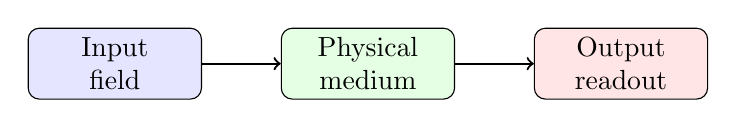
\begin{tikzpicture}[scale=0.9,
    box/.style={draw, rounded corners, minimum width=2.2cm, minimum height=0.9cm, align=center}]
\node[box, fill=blue!10] (in) {Input\\field};
\node[box, fill=green!10, right=1cm of in] (med) {Physical\\medium};
\node[box, fill=red!10, right=1cm of med] (out) {Output\\readout};
\draw[->, thick] (in) -- (med);
\draw[->, thick] (med) -- (out);
\end{tikzpicture}

\end{frame}

% ---------------------------------------------------------------------
\begin{frame}{Our workflow}

We tackle each computing primitive the same way:

\vspace{0.3cm}
\begin{enumerate}
    \item \textbf{Forward model} -- write a physics solver (FDTD, ODE, reaction-diffusion).
    \item \textbf{Task definition} -- choose inputs, readout probes, target outputs, and a loss.
    \item \textbf{Trainable design} -- decide what is tunable: geometry, rate constants, boundary conditions, or an external field.
    \item \textbf{Optimiser} -- wrap the forward solve in a gradient-free (or adjoint) loop.
    \item \textbf{Validation} -- check robustness, interpret the learned structure, and identify physical limits.
\end{enumerate}

\vspace{0.3cm}
\centering
The hard part is finding a physical system where this loop actually converges.

\end{frame}

% ---------------------------------------------------------------------
\begin{frame}{Avenues explored along the way}

\begin{table}
\centering
\footnotesize
\begin{tabular}{>{\raggedright\arraybackslash}p{2.5cm}>{\raggedright\arraybackslash}p{5.5cm}>{\raggedright\arraybackslash}p{2.5cm}}
\toprule
\textbf{Direction} & \textbf{What we looked at} & \textbf{Outcome} \\
\midrule
Poroacoustics / thermoviscous flow & Acoustic FDTD in porous media, JCA model, viscous heating & Losses dominate; control is hard \\
Recurrent chemical networks (RCN) & Dack-style fast/slow mass-action ODEs & XOR solved, but well-mixed \\
DNA / PEN enzyme networks & Strand-displacement and enzyme-based programmable reactions & Elegant, not spatially continuous \\
Reaction--diffusion & Gray-Scott, FitzHugh-Nagumo, Barkley, Oregonator & Spatial, trainable controls \\
\bottomrule
\end{tabular}
\end{table}

\vspace{0.2cm}
\centering
\footnotesize
Each avenue taught us something about what ``compute'' means in a physical medium.

\end{frame}
% ---------------------------------------------------------------------
\begin{frame}{acoustic wave computing}

Idea: sound waves propagating through structured solids/fluids interfere and route signals.

\vspace{0.2cm}
\begin{columns}[T]
\begin{column}{0.55\textwidth}
Governing equation:
\begin{align*}
    \frac{\partial^2 p}{\partial t^2} = c^2 \nabla^2 p
\end{align*}

\vspace{0.1cm}
\begin{itemize}
    \footnotesize
    \item Frequency-dependent transmission through obstacle arrays.
    \item Bragg gratings and porous media give tunable dispersion.
    \item Thermoviscous losses and fabrication/control are hard.
\end{itemize}
\end{column}
\begin{column}{0.42\textwidth}
\centering

\includegraphics[width=\textwidth]{../small_spacing_sweep_fixed.png}
\end{column}
\end{columns}

\vspace{0.2cm}
\centering
\footnotesize
Result: a working FDTD solver, but the feasibility of a \textit{trainable} device was unclear.

\end{frame}

% ---------------------------------------------------------------------
\begin{frame}{RCN result: a trainable chemical ODE}

Dack-style recurrent chemical network: fast perceptron species $Y_j$ plus slow executive species $X_i$.

\vspace{0.2cm}
\begin{columns}[T]
\begin{column}{0.58\textwidth}
\begin{align*}
    \frac{dX_i}{dt} &= \beta_i + X_i \sum_j \alpha_{ij} Y_j \\
    \mu \frac{dY_j}{dt} &= \gamma + \theta_j Y_j + Y_j \sum_i \omega_{ji} X_i - Y_j^2
\end{align*}

\vspace{0.1cm}
\footnotesize
Result: a well-mixed mass-action ODE can learn XOR.\\
Limitation: no spatial continuity; trainable parameters are rate constants.
\end{column}
\begin{column}{0.40\textwidth}
\centering
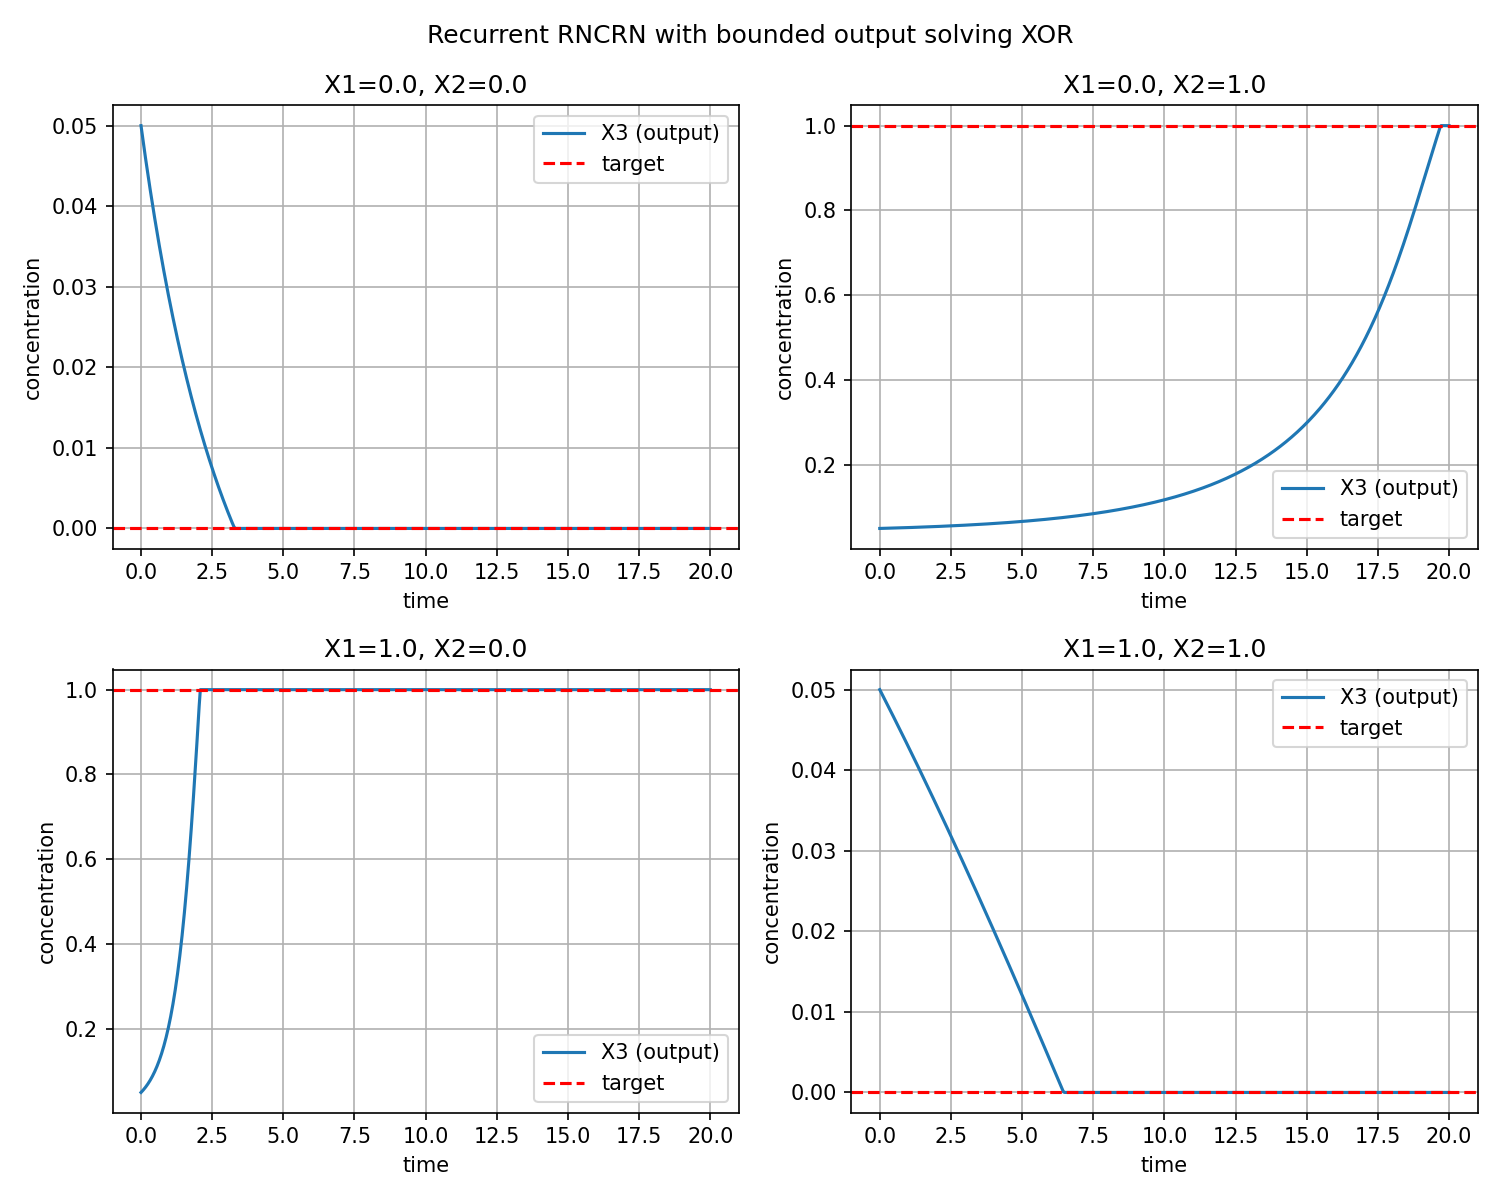
\includegraphics[width=\textwidth]{../Analysis/dack_rncrn_xor_recurrent_bounded_results.png}
\end{column}
\end{columns}

\end{frame}

% ---------------------------------------------------------------------
\begin{frame}{reaction-diffusion computing}

Idea: use excitable chemical media where waves propagate, collide, and diffract.

\vspace{0.2cm}
\begin{columns}[T]
\begin{column}{0.55\textwidth}
\small
Oregonator model:
\begin{align*}
    \frac{\partial u}{\partial t} &= D_u \nabla^2 u + \frac{1}{\varepsilon}\left[ u - u^2 - (f v + \phi)\frac{u-q}{u+q} \right] \\
    \frac{\partial v}{\partial t} &= D_v \nabla^2 v + u - v
\end{align*}

\vspace{0.1cm}
\footnotesize
\begin{itemize}
    \item $u \sim$ HBrO$_2$, $v \sim$ oxidised catalyst.
    \item $\phi(x,y)$ is a light-suppression field; geometry and $\phi$ are trainable controls.
\end{itemize}
\end{column}
\begin{column}{0.44\textwidth}
\centering
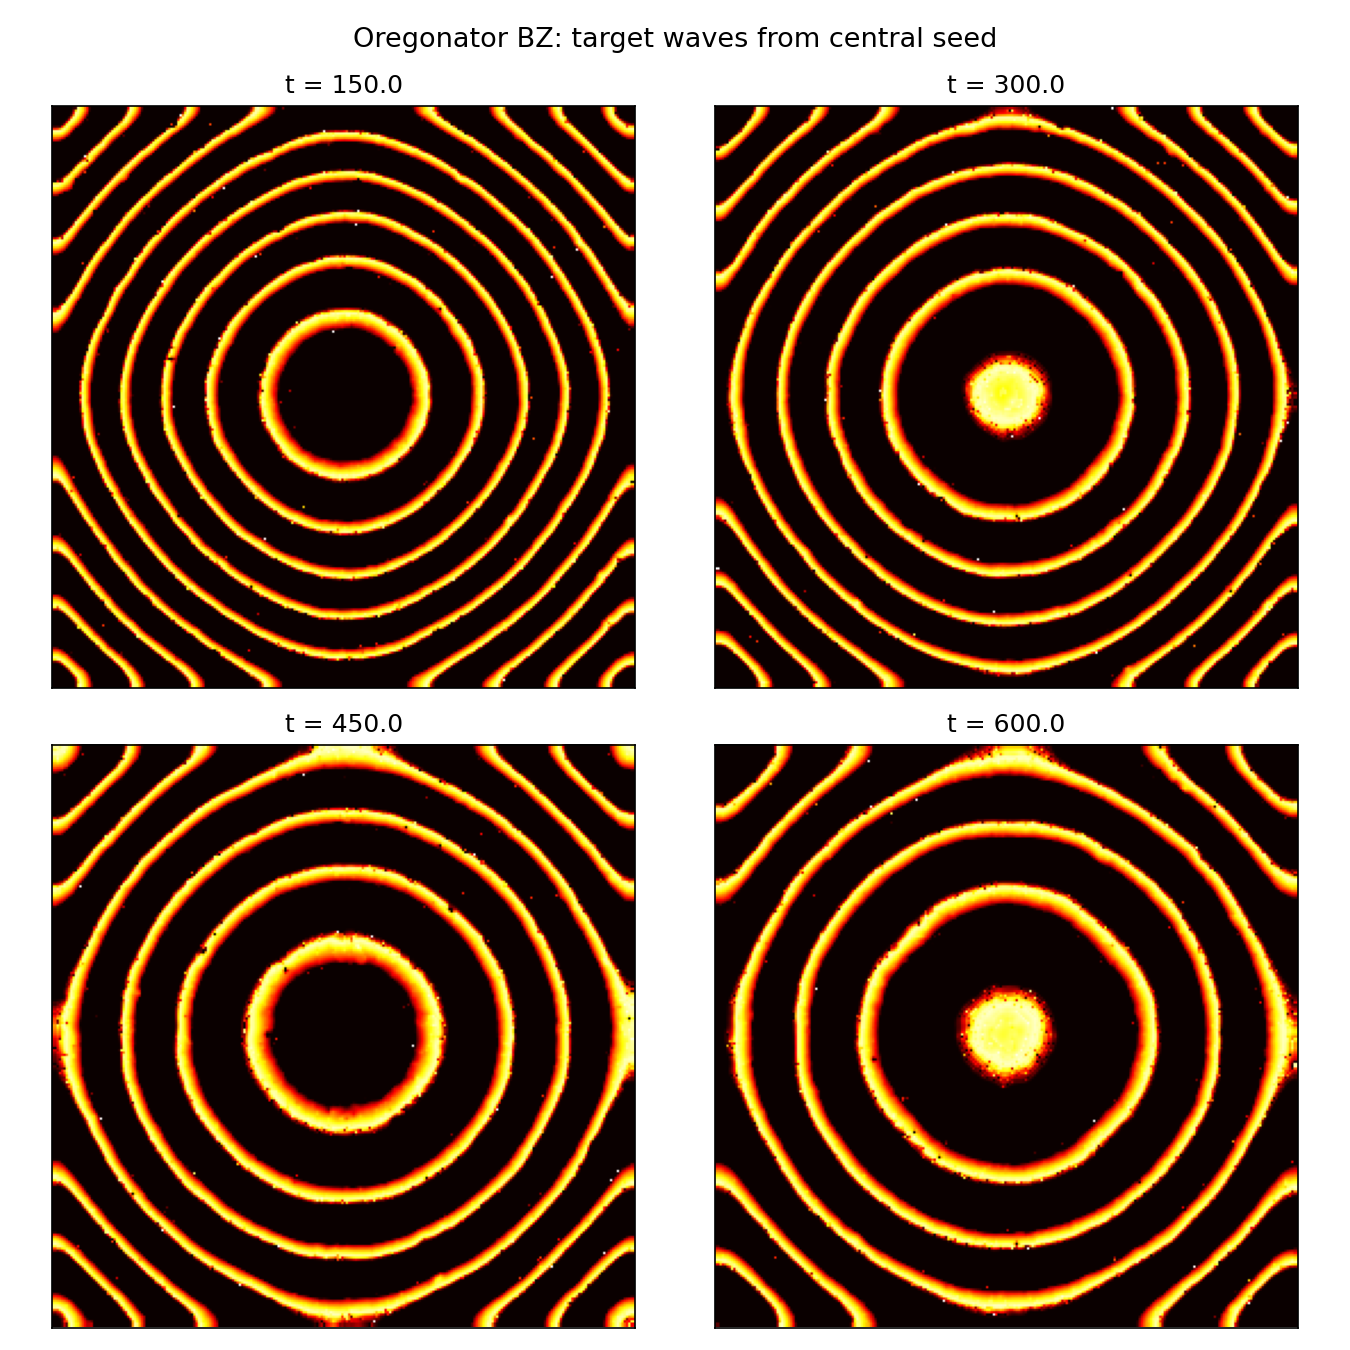
\includegraphics[width=0.48\textwidth]{../Analysis/oregonator_target.png}
\hfill
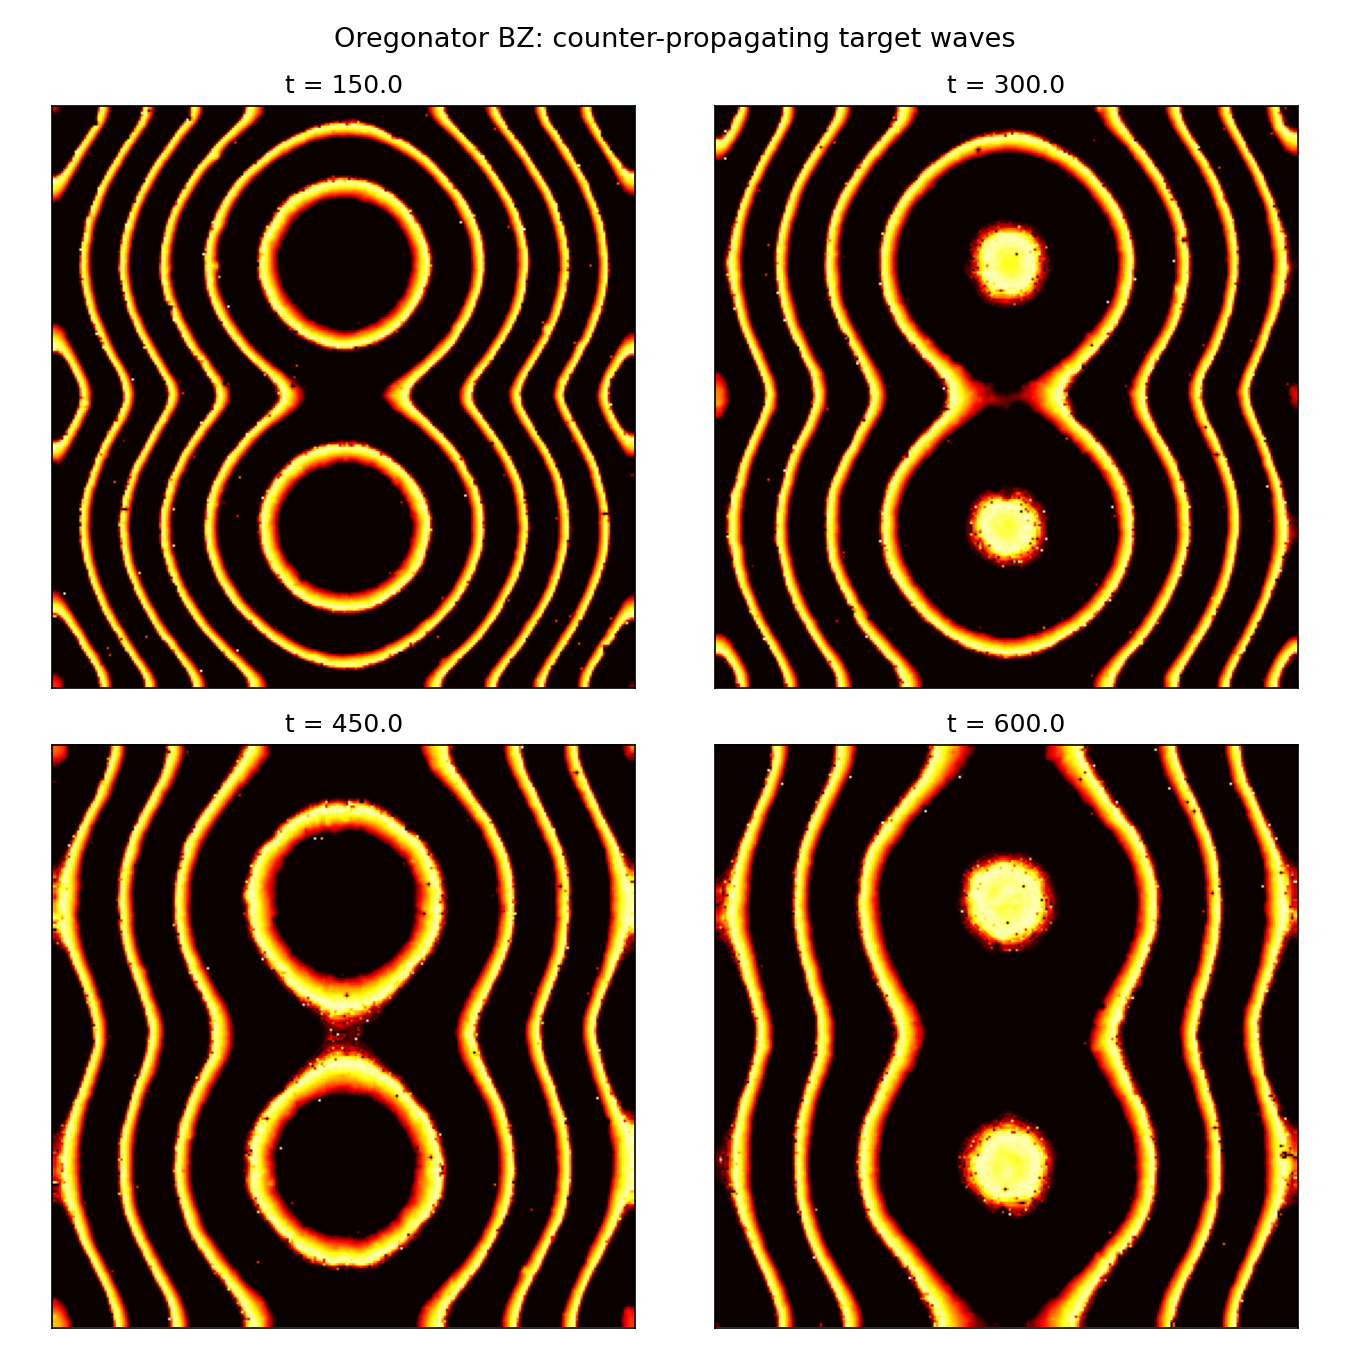
\includegraphics[width=0.48\textwidth]{../Analysis/oregonator_collision.png}

\vspace{0.1cm}
{\footnotesize Target waves \hfill Collision / annihilation}
\end{column}
\end{columns}

\end{frame}
% ---------------------------------------------------------------------
\begin{frame}{Current status and the open question}

What we have now:
\begin{itemize}
    \item A robust 2D Oregonator forward solver.
    \item Waves that route, collide, and diffract through gaps.
    \item Timing of input pulses adds another controllable degree of freedom.
\end{itemize}

\vspace{0.3cm}
\centering
\textbf{Open question:} can we train geometry or an excitability map so these waves implement a logic gate?

\vspace{0.3cm}
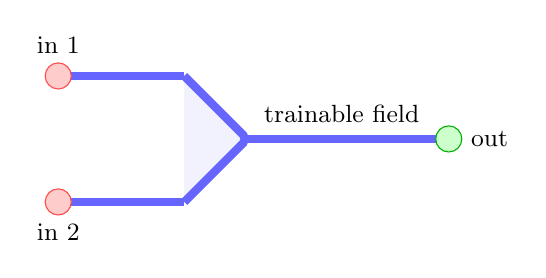
\begin{tikzpicture}[scale=0.8,
    channel/.style={draw=blue!60, line width=3pt, rounded corners=2pt, fill=blue!5},
    input/.style={draw=red!70, fill=red!20, circle, minimum size=6pt},
    output/.style={draw=green!70!black, fill=green!20, circle, minimum size=6pt}]

\draw[channel] (0,2) -- (2,2);
\draw[channel] (0,0) -- (2,0);
\draw[channel] (2,2) -- (3,1) -- (2,0);
\draw[channel] (3,1) -- (6,1);

\node[input] at (0,2) {};
\node[input] at (0,0) {};
\node[output] at (6.2,1) {};
\node[above] at (0,2.2) {\small in 1};
\node[below] at (0,-0.2) {\small in 2};
\node[right] at (6.4,1) {\small out};
\node at (4.5,1.4) {\small trainable field};
\end{tikzpicture}

\end{frame}

\end{document}
